\section{Looking at the big picture}
\label{sec:ch2:bigpicture}


Welcome to the Neurobiology Institute! A research advisor you work for has come to you with an interesting problem. The brains of organisms consist of neurons, which are individual cells which have a rather complex functions. Different patterns in which these neurons connect produce the unique functions your brain is able to do: it is able to manage passive functions like breathing, a heartbeat, vascular tone (the ability of your blood vessels to contract and relax to keep blood pumping through your body), as well as more active functions like moving, hearing, seeing, and higher level thought like your ability to read this book or remember the content.

In a simplified explanation, the way these neurons work is that, when they are electrically stimulated, they transmit that electrical signal to other neurons. This process consumes a lot of energy for your body; while the brain is only about 2\% of your total body weight, it consumes about 20\% of the energy your body uses per day. To keep the neurons replenished with energy (and to remove waste that the cells produce when they work), the brain has a complicated network of blood vessels. When a brain area is in use, the body dedicates blood supply to the area that will need it most.

Through this biological mechanism, neurobiologists came up with a rather clever way to decipher brain activity in humans. With the use of magnetically sensitive contrasts that lie in the blood, they found that when a person sits for a magnetic resonance imaging (MRI) session, that they could pick up the particular areas that the blood was flowing towards. Scientists were able to trace this signal, and over the course of several years, they were able to decipher that this signal really did, in fact, tend to correlate with brain activity. 

\begin{figure}[h]
    \centering
    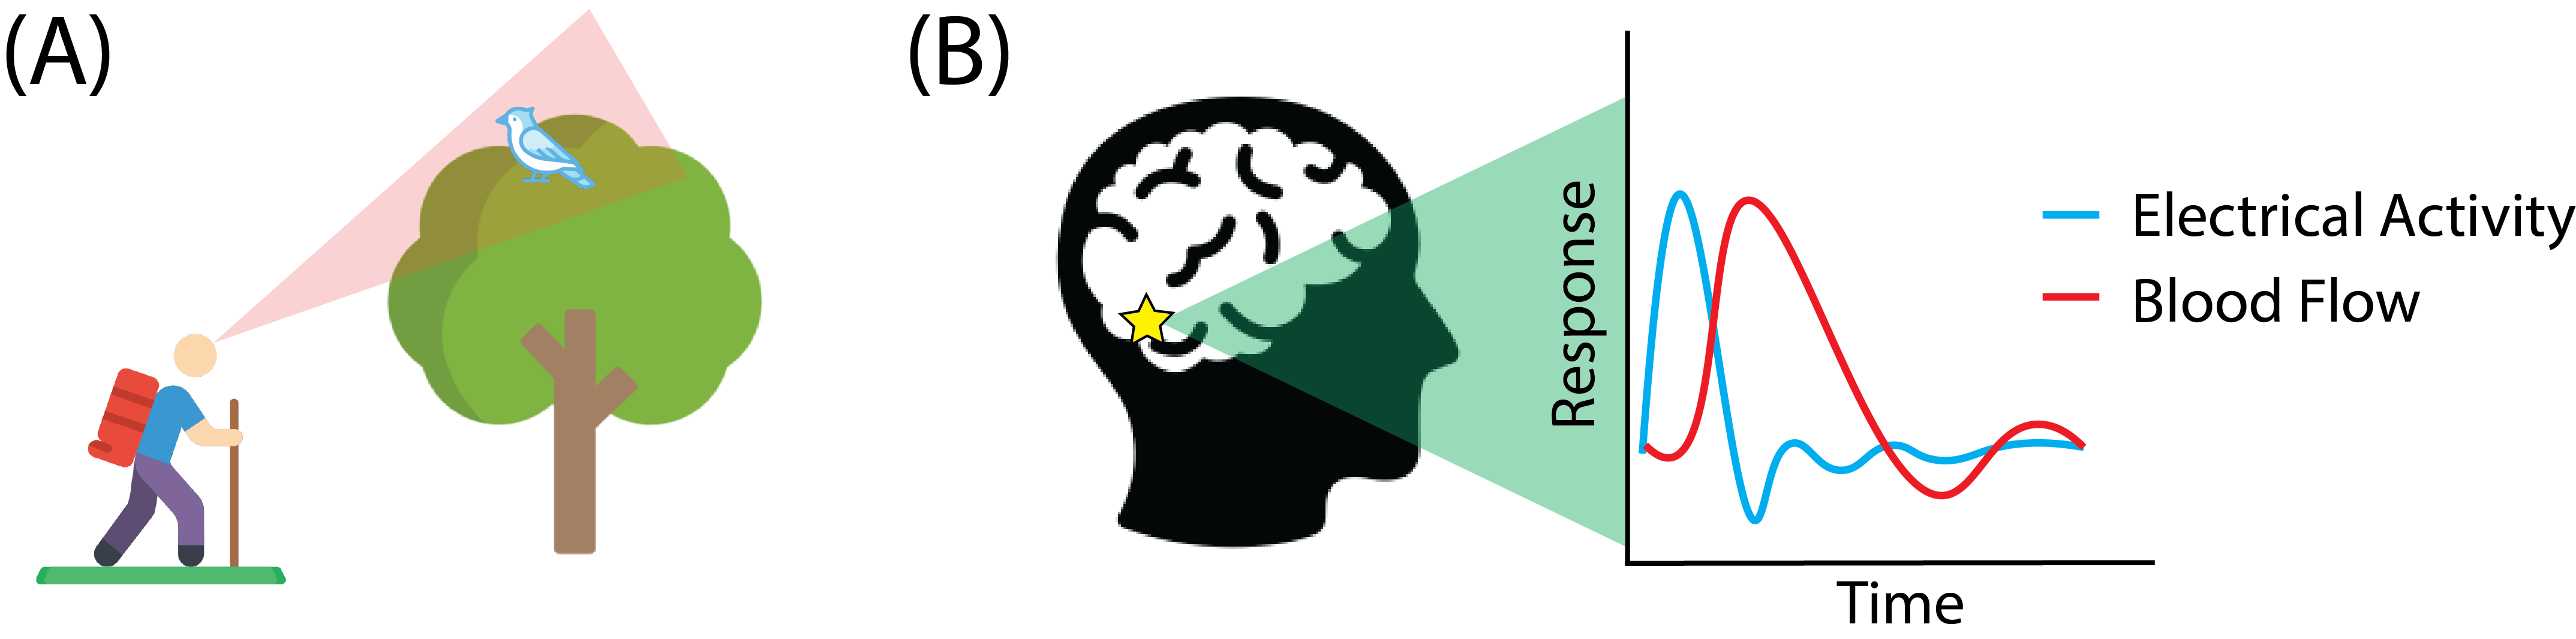
\includegraphics[width=\linewidth]{foundations/ch2/Images/fmri_bold.png}
    \caption[BOLD f-MRI]{(A) A hiker out on the trails sees a bird pirched in a tree in his field of view (faint red triangle). (B) The occipital lobe, which is responsible for sight, sits in the back of the brain (star). The presence of the bird in the field of view causes neurons to be electrically stimulated (blue line). The activity of the neurons causes the brain to send blood to the area as the neurons are stimulated (red line). While individual neurons are too small to see, the blood flow of many neurons in the brain can be picked up by the fMRI scanner.}
    \label{fig:fmri-bold}
\end{figure}

This imaging technology, known as functional MRI (fMRI, \emph{functional} because it images brain regions as they \emph{function}) has proven to be extremely interesting to neuroscientists \cite{Poldrack2011Aug}. Basically, people sit in a big fMRI machine, and the scanner simply looks at this blood signal over time in different areas of the brain. For a given pair of brain areas, the researchers look at whether the two areas tend to be active together. Stated another way, they look for \emph{correlations} that arise between different brain areas. The idea is that, perhaps, different combinations of brain areas tend to work together as a unit, allowing the complicated thought patterns that humans are capable of. By viewing the different areas of the brain as nodes of a network, and the correlations as the edges, scientists have constructed networks from this line of thinking. This area of study, called connectomics, presents an extremely network-centric area of research \cite{Munsell2018Sep}.

One of your colleagues has come to you with an interesting question. He has a bunch of networks from fMRI sessions, and he wants to know whether there are any higher level groups of brain areas that tend to have similar activity. He comes to you with a question: can you, as a network scientist, take his network of nodes and edges, and figure out a way to break the nodes into groups of nodes which are functionally similar?

If these are the types of questions you have when you see new network data, then this is the right book for you. 

\subsection{Framing the problem}

The first question to ask your colleague is; what exactly is the objective here? How will science (or a company) use and benefit from the knowledge we hope to gain? In network machine learning, the choice of the model used is \emph{everything}. The model determines what sorts of questions we are capable of asking, and what sorts of \emph{answers} we are capable of learning. Asking about the objectives will directly shape which models and approaches you use.

Your colleague replies that he will give you a bunch of networks. The networks will be the functional brain network from human beings, where nodes will be regions of the brain from an MRI scan. The edge weights in the network will represent how correlated the brain activity is for each pair of brain areas. Your colleague wants to know whether there are any sub-groups of areas that tend to behave similarly. By ``behave similarly'', what your colleague means is, are there sub-groups of brain areas that tend to work together in conjunction with other sub-groups of brain areas?

The next question to ask is what the current solution looks like. This will help you to understand where to start approaching the problem, and give you a reference for the performance of your techniques. Your colleague answers that he thinks that some people use a thing called spectral embedding methods, and he wants to know whether you might be able to do something similar. 

Next, you need to determine what type of network machine learning problem you have. What type of data do you have? Do you have any covariates associated with that data? What type of question do you want to answer? Do you want to test a hypothesis, or make predictions? What characteristics will your model need to reflect to be able to answer the question appropriately? Before you progress further, you should try to think and answer these questions for yourself. 

Remembering back to the types of network machine learning problems in Section \ref{sec:ch1:types}, you immediately conclude that this is a multiple network learning problem. Your networks are non-attributed, since you only know the nodes and edges of the network. The question asks about groups of nodes and edges, and you hope to use network modelling approaches to study your problem. You are going to need to come up with a definition of what it means for pairs of areas to be similar, and you are going to want to be able to group areas in a way that is meaningful for your colleague.

\subsection{Check the assumptions}

Throughout the course of this book, we will try to keep in direct focus the assumptions being made by the techniques you might pick. You want to choose the simplest set of assumptions that can reasonably reflect the data. This means that you want to use the simplest statistical model that can answer the question you want to address. In this case, we don't care about individual brain area-to-brain area connections at all: we only care about how groups of brain areas behave in relation to other groups of brain areas. This means that we want to choose models which will allow us to learn about pairs of brain area groups, which is a very different problem from learning about individual brain areas themselves. You don't want to find out after developing an analysis which produces results on pairs of brain area groups that your boss actually wanted you to compare individual brain areas themselves!

After talking over your understanding of the problem with your research colleague, you are confident that he wants a way to be able to group brain areas together based on how similar they are, and he gives you freedom to define that however you choose. You now have the green light to get coding!

\newpage